\documentclass[11pt, oneside]{article} 
\usepackage{geometry}
\geometry{letterpaper} 
\usepackage{graphicx}
	
\usepackage{amssymb}
\usepackage{amsmath}
\usepackage{parskip}
\usepackage{color}
\usepackage{hyperref}

\graphicspath{{/Users/telliott/Github/figures/}}
% \begin{center} \includegraphics [scale=0.4] {gauss3.png} \end{center}

\title{Sum of integers}
\date{}

\begin{document}
\maketitle
\Large

%[my-super-duper-separator]

\label{sec:sum_of_integers}

In calculus, we will compute Riemann sums, and to do that we need to find formulas for the sum of squared integers, cubed integers, and so on.  To keep it simple, let's start with the integers from $1$ to $n$.

In a previous chapter we introduced the method called induction.  Probably the most famous example of an inductive proof is that for the sum of integers.
\[ S_n = 1 + 2 + \dots + n \]

\emph{Proof}.

The numbers we seek are called the triangular numbers.  These are
\[ 1, 3, 6, 10 \cdots \]
These are generated as the third diagonal of Pascal's triangle.:

\begin{center} 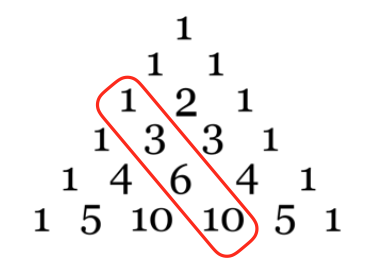
\includegraphics [scale=0.4] {pascal2.png} \end{center}

Suppose someone has sent us, anonymously, a formula which they claim gives the sum of the first $n$ integers, namely 

\[ S_n = \frac{n (n + 1)}{2} \]

Assume the formula is correct for $S_n$.  Add $n+1$ to both sides.  The left-hand side becomes $S_{n+1}$, so we have:
\[ S_{n + 1} = \frac{(n)(n + 1)}{2} + (n+1) \]

Rearranging:
\[ = \frac{n(n + 1) + 2(n + 1)}{2} \]
\[ = \frac{(n + 1)(n + 2)}{2} \]

which is exactly what we'd get by substituting $n+1$ for $n$ in the original formula.

Alternatively, sometimes it's clearer to assume the $n-1$ case and prove the formula is correct for $n$:
\[ S_{n-1} = \frac{n(n-1)}{2} \]
\[ S_n = \frac{n(n-1)}{2} + n \]
\[ = \frac{n(n-1) + 2n}{2} \]
\[ = \frac{n(n-1 + 2)}{2} = \frac{n(n + 1)}{2} \]

So we have proven that if the $S_n$ formula is correct, then so is the one for $S_{n+1}$.

How do we know that $S_n$ is correct?

Just check the \emph{base case}:
\[ S_1 = \frac{1(1 + 1)}{2} = 1 \]
Since $S_1$ is clearly correct, $S_2$ must be also, and this continues all the way to $S_{n}$.
\[ S_1 \Rightarrow S_2 \Rightarrow \dots S_{n-1} \Rightarrow S_n \Rightarrow S_{n+1} \]

Therefore, it must be true for \emph{every} integer $n$.

$\square$

There is a famous story about Gauss.  As a schoolboy, he "saw" how to add the integers from $1$ to $100$ as two parallel sums.

\begin{center} 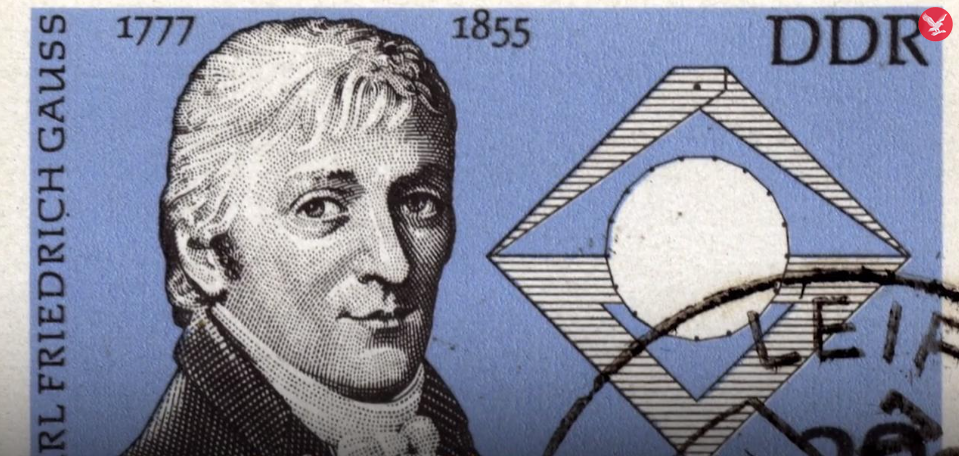
\includegraphics [scale=0.25] {gauss4.png} \end{center}
Added together horizontally, these two series must equal twice the sum of $1$ to $100$.  

But vertically, we notice that each sum is equal to $n+1$, and we have $n$ of them.  
\begin{center} 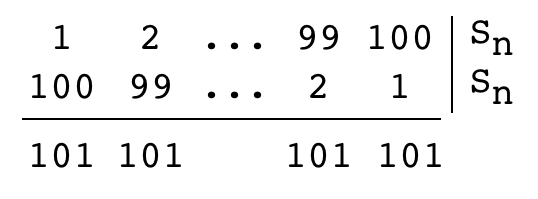
\includegraphics [scale=0.40] {gauss_sum.png}\end{center}

So, again
\[ 2S_n = n (n+1) \]
\[ S_n = \frac{1}{2} \ n (n+1) \]
For $n=100$ the value of the sum is $5050$, which is what Gauss wrote on his slate and presented to the teacher immediately on being given the problem as a make-work exercise.

One way of looking at this result is that between $1$ and $100$ there are $100$ representatives of the "average" value in the sequence, which (because of the monotonic steps) is $(100 + 1)/2 = 50.5$.  

Or alternatively, view the sum as ranging from $0$ to $100$ (with the same answer).  Now there are $101$ examples of the average value ($100 + 0)/2 = 50$).

\subsection*{proof without words}

Here is a striking \emph{visual proof} of the formula to obtain T$_n$, the $n^{th}$ such number.  The total number of circles in the figure below is $n \times (n+1)$ and this is exactly two times the sum of the integers from $1$ to $n$.

\begin{center} 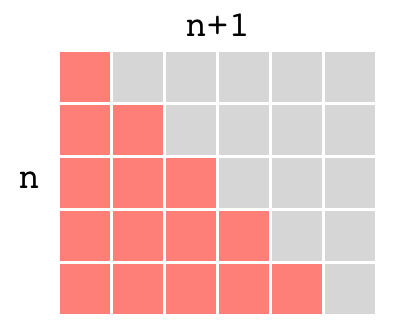
\includegraphics [scale=0.35] {int_sum2.png}\end{center}
\[ 2S = n(n+1) \]

\subsection*{Derivation using sums}
It seems a shame to spoil such a beautiful proof "without words" as the one above by saying anything more, but I can't resist.  I'd like to derive the equation we have been using using algebra.  The general method will help us later.

For any number, and in particular, any integer $k$ it is true that
\[ (k+1)^2 = k^2 + 2k + 1 \]
So consider what happens if we sum the values from $k=1 \rightarrow n$ for each of these terms
\[ \sum_{k=1}^n (k+1)^2 = \sum_{k=1}^n k^2 + \sum_{k=1}^n 2k + \sum_{k=1}^n 1 \]

If the equation is valid for any individual $k$, then the sum is also valid, plugging in all $k$ up to $n$.

Rearranging
\[ \sum_{k=1}^n (k+1)^2 - \sum_{k=1}^n k^2 = \sum_{k=1}^n 2k + \sum_{k=1}^n 1 \]
Now think about the left-hand side in our equation. 
\[ \sum_{k=1}^n (k+1)^2 - \sum_{k=1}^n k^2 \]

We have a bunch of terms starting with $2^2$:
\[ 2^2 + 3^2 + \dots + n^2 + (n+1)^2 \]
we also have a bunch of terms to subtract starting with $1^2$:
\[ 1^2 + 2^2 + 3^2 + \dots + n^2 \]
Almost everything cancels.  This is called a "collapsing" or "telescoping" sum.  We have
\[ (n+1)^2 - 1 = n^2 + 2n \]

Bringing back the right-hand side  we obtain:
\[ n^2 + 2n = \sum_{k=1}^n 2k + \sum_{k=1}^n 1 \]
We can bring the constant factor $2$ out of the sum, and also, we recognize that the sum of the value $1$ a total of $n$ times is just $n$.
\[ n^2 + 2n = 2\sum_{k=1}^n k + n \]

Subtract $n$ from both sides and divide by $2$:
\[ \sum_{k=1}^n k = \frac{n (n+1)}{2} \]
That's it!

\end{document}